\documentclass[12pt,a4paper]{article}
\usepackage[UTF8]{ctex}
\usepackage{amsmath,amssymb}
\usepackage{xcolor}
\usepackage{hyperref}
\usepackage{geometry}
\usepackage{graphicx}
\geometry{margin=2.5cm}

\title{Discrete Logarithm / 离散对数}
\author{QuoNic}
\date{}

\begin{document}
\maketitle

\begin{center}
\textbf{Algorithms / 算法} | 难度：高级 | 预计时间：25 分钟
\end{center}

\tableofcontents
\newpage

\section{为什么需要？}

离散对数问题是密码学的基础，量子算法可以高效求解。

\subsection{经典局限}
\begin{itemize}
  \item 经典算法需要指数时间，对于 $n$ 位数需要 $O(\exp(\sqrt{n}))$ 时间
  \item 对于大数，经典方法效率低
  \item 经典算法无法利用量子并行性
\end{itemize}

\subsection{量子优势}
\begin{itemize}
  \item 量子算法可以在多项式时间内求解，对于 $n$ 位数需要 $O(n^3)$ 时间
  \item 提供指数加速
  \item 是量子密码学的基础
\end{itemize}

\subsection{实际应用}
\begin{itemize}
  \item 密码学（Diffie-Hellman 密钥交换）
  \item 数字签名（DSA、ECDSA）
  \item 椭圆曲线密码学
\end{itemize}

\section{快速上手}

\begin{verbatim}
from quonic.algorithms import discrete_log

# 求解离散对数：2^x ≡ 8 (mod 11)
result = discrete_log(g=2, h=8, p=11)
print(f'x = {result.x}')
\end{verbatim}

\textbf{预期输出}：
\begin{verbatim}
x = 3
\end{verbatim}

\section{原理详解}

\subsection{电路图}

\begin{center}
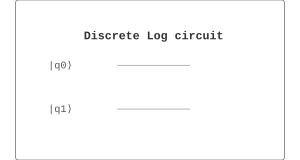
\includegraphics[width=0.6\textwidth]{../../images/discrete_log_circuit.svg}
\end{center}

\subsection{数学推导}

\textbf{Step 1: 问题定义}

给定 $g, h, p$，求 $x$ 使得：
\begin{equation}
g^x \equiv h \pmod{p}
\end{equation}

\textbf{Step 2: 量子算法}

使用 Shor 算法的变体：
\begin{enumerate}
  \item 选择随机 $a$
  \item 用 QPE 估计 $g^a \mod p$ 的阶 $r$
  \item 计算 $x = a \cdot r^{-1} \mod (p-1)$
\end{enumerate}

\textbf{Step 3: QPE 估计阶}

QPE 估计阶 $r$：
\begin{equation}
|0\rangle|1\rangle \to \sum_k |k\rangle|g^k \mod p\rangle
\end{equation}

测量第一个寄存器得到 $k$，用连分数展开求 $r$。

\textbf{Step 4: 经典后处理}

计算离散对数：
\begin{equation}
x = a \cdot r^{-1} \mod (p-1)
\end{equation}

\subsection{几何解释}

离散对数在有限域上求解，利用量子傅里叶变换提取周期信息。

\section{代码详解}

\begin{verbatim}
from quonic.algorithms import discrete_log

# discrete_log(g, h, p)
# g: 生成元
# h: 目标值
# p: 模数

result = discrete_log(g=2, h=8, p=11)

# result.x: 离散对数
# result.period: 阶
# result.circuit: 量子电路
print(f'x = {result.x}')
print(f'Period: {result.period}')
\end{verbatim}

\section{进阶用法}

\subsection{场景 1：不同参数}

\begin{verbatim}
from quonic.algorithms import discrete_log

# 不同参数
result = discrete_log(g=3, h=27, p=13)
print(f'x = {result.x}')
\end{verbatim}

\subsection{场景 2：大数}

\begin{verbatim}
from quonic.algorithms import discrete_log

# 大数
result = discrete_log(g=2, h=1024, p=1031)
print(f'x = {result.x}')
\end{verbatim}

\section{适用场景}

\subsection{密码学}

离散对数是许多密码系统的基础，如 Diffie-Hellman 密钥交换。

\subsection{数字签名}

DSA 和 ECDSA 基于离散对数问题。

\subsection{椭圆曲线密码学}

椭圆曲线离散对数问题是椭圆曲线密码学的基础。

\section{常见问题}

\subsection{离散对数和大数分解有什么关系？}

都基于周期查找问题，可以用 Shor 算法求解。

\subsection{量子算法的加速比是多少？}

指数加速：$O(\text{poly}(\log N))$ vs $O(\exp(\sqrt{\log N}))$。

\subsection{离散对数问题的难度如何？}

离散对数问题是 NP-hard 的，但不是 NP-complete 的。

\section{学习路径}

\subsection{前置知识}
\begin{itemize}
  \item Shor 算法
  \item 量子傅里叶变换
  \item 数论
\end{itemize}

\subsection{继续学习}
\begin{itemize}
  \item 椭圆曲线密码学
  \item 后量子密码学
  \item 量子密码学
\end{itemize}

\section{完整示例代码}

\subsection{示例 1：基本离散对数}

\begin{verbatim}
from quonic.algorithms import discrete_log

result = discrete_log(g=2, h=8, p=11)
print(f'x = {result.x}')
\end{verbatim}

\section{下载}

\begin{itemize}
  \item [discrete\_log.py](https://github.com/ChrisLee0721/QuoNic/blob/main/examples/discrete_log/discrete_log.py)
\end{itemize}

\end{document}
